% Copyright 2004 by Till Tantau <tantau@users.sourceforge.net>.
%
% In principle, this file can be redistributed and/or modified under
% the terms of the GNU Public License, version 2.
%
% However, this file is supposed to be a template to be modified
% for your own needs. For this reason, if you use this file as a
% template and not specifically distribute it as part of a another
% package/program, I grant the extra permission to freely copy and
% modify this file as you see fit and even to delete this copyright
% notice. 

\documentclass{beamer}

% \usepackage{natbib}
\usepackage{times}
% There are many different themes available for Beamer. A comprehensive
% list with examples is given here:
% http://deic.uab.es/~iblanes/beamer_gallery/index_by_theme.html
% You can uncomment the themes below if you would like to use a different
% one:
%\usetheme{AnnArbor}
%\usetheme{Antibes}
%\usetheme{Bergen}
%\usetheme{Berkeley}
%\usetheme{Berlin}
%\usetheme{Boadilla}
%\usetheme{boxes}
%\usetheme{CambridgeUS}
%\usetheme{Copenhagen}
%\usetheme{Darmstadt}
%\usetheme{default}
%\usetheme{Frankfurt}
%\usetheme{Goettingen}
%\usetheme{Hannover}
%\usetheme{Ilmenau}
%\usetheme{JuanLesPins}
%\usetheme{Luebeck}
\usetheme{Madrid}
%\usetheme{Malmoe}
%\usetheme{Marburg}
%\usetheme{Montpellier}
%\usetheme{PaloAlto}
%\usetheme{Pittsburgh}
%\usetheme{Rochester}
%\usetheme{Singapore}
%\usetheme{Szeged}
%\usetheme{Warsaw}

\title{The Shortest Path in Line Arrangements}

% A subtitle is optional and this may be deleted
% \subtitle{Optional Subtitle}z

\author{Ligeng Zhu\inst{1} }
% - Give the names in the same order as the appear in the paper.
% - Use the \inst{?} command only if the authors have different
%   affiliation.

\institute[Simon Farser University] % (optional, but mostly needed)
{
  \inst{1}%
  Department of Computing Science\\
  Simon Fraser University
  % \and
  % \inst{2}%
  % Department of Theoretical Philosophy\\
  % University of Elsewhere
}
% - Use the \inst command only if there are several affiliations.
% - Keep it simple, no one is interested in your street address.

\date{CMPT 406, 2017 Fall}
% - Either use conference name or its abbreviation.
% - Not really informative to the audience, more for people (including
%   yourself) who are reading the slides online

\subject{Theoretical Computer Science}
% This is only inserted into the PDF information catalog. Can be left
% out. 

% If you have a file called "university-logo-filename.xxx", where xxx
% is a graphic format that can be processed by latex or pdflatex,
% resp., then you can add a logo as follows:

% \pgfdeclareimage[height=0.5cm]{university-logo}{university-logo-filename}
% \logo{\pgfuseimage{university-logo}}

% Delete this, if you do not want the table of contents to pop up at
% the beginning of each subsection:
\AtBeginSubsection[]
{
  \begin{frame}<beamer>{Outline}
    \tableofcontents[currentsection,currentsubsection]
  \end{frame}
}

% Let's get started
\begin{document}

\begin{frame}
  \titlepage
\end{frame}

\begin{frame}{Outline}
  \tableofcontents
  % You might wish to add the option [pausesections]
\end{frame}

\section{Problem Definition}

\begin{frame}{Problem Definition}{}
    \begin{tabular}{c c}
        \begin{minipage}{0.4\textwidth}
            \begin{center}
                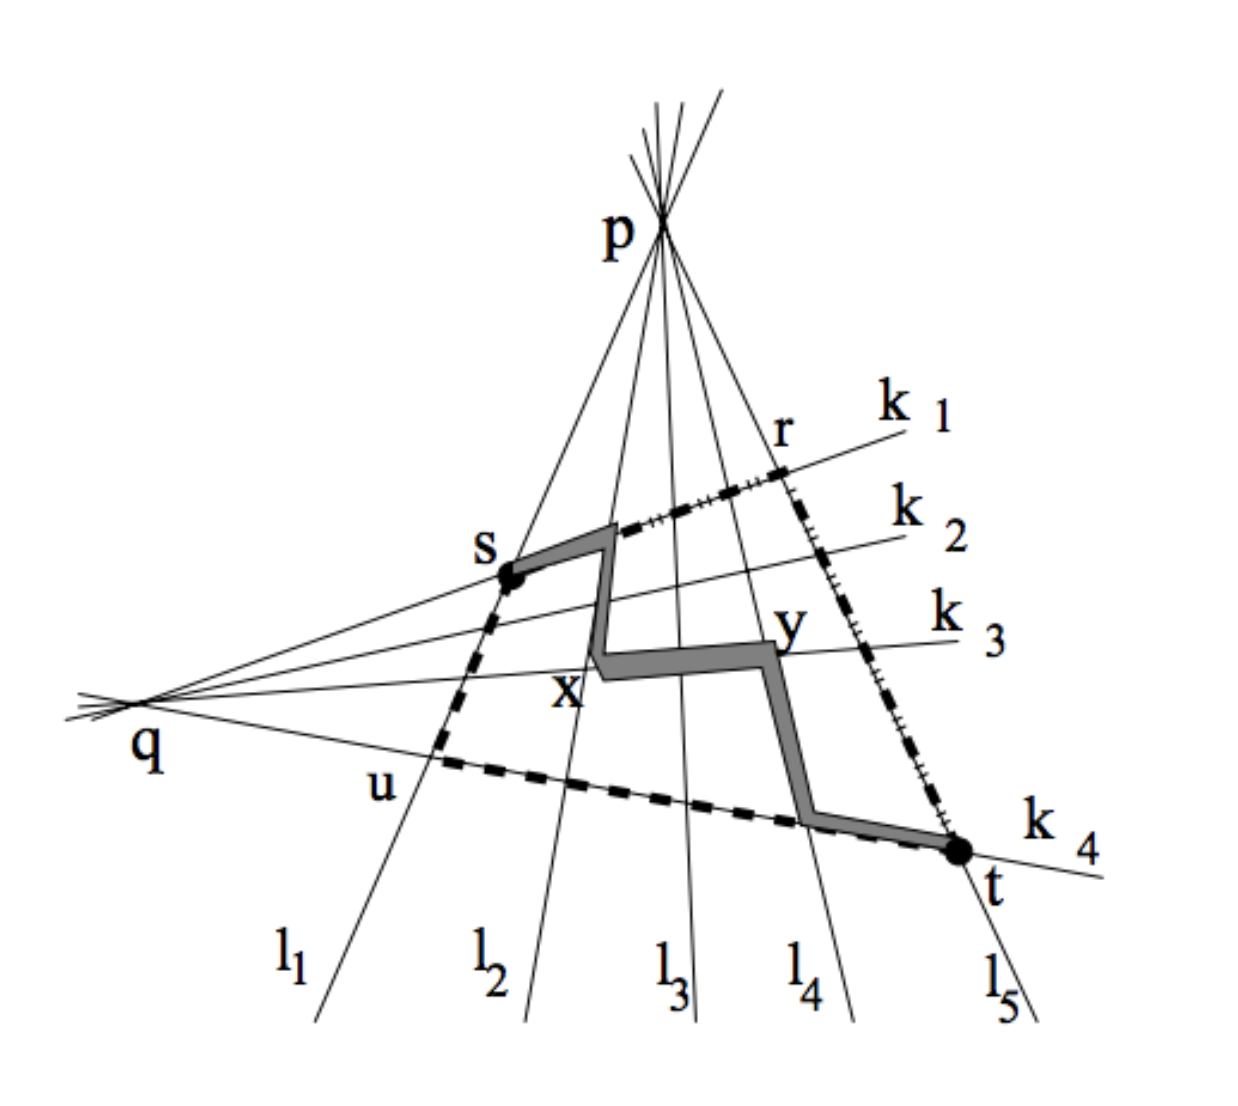
\includegraphics[width=\linewidth]{problem_definition.png}
            \end{center}
        \end{minipage}  
        &  
        \begin{minipage}{0.5\textwidth}
            By given lines from two centrals, compute the shortest path between extreme up-left point $s$ and extrem right-bottom point $t$. 
        \end{minipage} 
    \end{tabular}
  
\end{frame}

% Section and subsections will appear in the presentation overview
% and table of contents.
\section{Related Works}
% \subsection{Planar Graph }

\begin{frame}{Related Works}{Shortest Path on Planar Graph}
  \begin{theorem} 
    The shortest path in a planar graph is $O(n^2)$. \cite{henzinger1997faster}
  \end{theorem}
  \begin{center}
    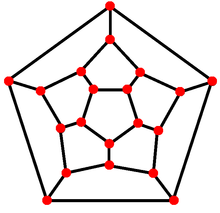
\includegraphics[width=0.3\linewidth]{planar.png}
  \end{center}
  Planar graph: edges do not intersect.
\end{frame}


\begin{frame}{Related Works}{Shortest Path on Planar Graph}
    \begin{tabular}{c c}
        \begin{minipage}{0.3\textwidth}
            \begin{center}
                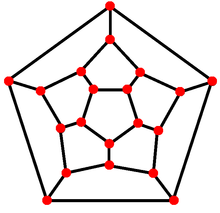
\includegraphics[width=\linewidth]{planar.png}
            \end{center}
        \end{minipage}  
        &  
        \begin{minipage}{0.6\textwidth}
            Simple proof: 
                 $$dist[s, t] = min(dist[s, m] + dist[m, t])$$
                 $$\forall \text{m, t is connected}$$
            Each edge is considered at most twice. \\
                 $$O(|E|) = O(n^2)$$
        \end{minipage} 
    \end{tabular}
\end{frame}

% \subsection{Special case: only vertical and horizontal}
% You can reveal the parts of a slide one at a time
% with the \pause command:


\begin{frame}{Related Works}{Special case: only vertical and horizontal}
   \begin{center}
    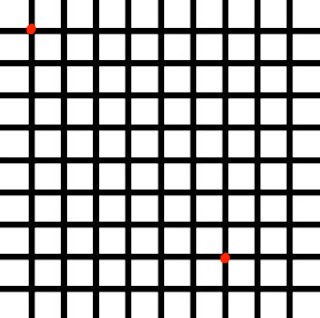
\includegraphics[width=0.3\linewidth]{grid2.jpg}
  \end{center}
  \begin{theorem} 
    The shortest path in a grid graph is $O(n^{1.5})$. \cite{eppstein1997efficient}
  \end{theorem}
  \begin{theorem} 
    The special case can be further improved to $O(nlgn)$.  M. van Kreveld
  \end{theorem}
\end{frame}


\begin{frame}{Related Works}{Special case: only k-slope}
%   \begin{center}
%     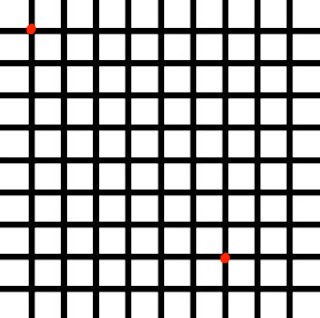
\includegraphics[width=0.3\linewidth]{grid2.jpg}
%   \end{center}
  \begin{theorem} 
    The shortest path with k-slope line arrangements is $O(n + k^2)$. \cite{eppstein1999shortest}
  \end{theorem}
  Note: $k$ can be as worse as $2 \times n$.
\end{frame}


\begin{frame}{Related Works}{Randomization approach }
  \begin{theorem} 
    The shortest path in a grid graph has $2$ approximation that runs in $O(nlgn)$ time. \cite{hart2001approximating}
  \end{theorem}
  Note: Find the shortest path on dual problem.
  \begin{theorem} 
    The shortest path in a grid graph has $1 + \epsilon$ approximation of SPLA in time $O(nlogn + min(n, \frac{1}{\epsilon^2}) + \frac{1}{\epsilon} log \frac{1}{\epsilon})$
  \end{theorem}
  Note: very, very complex. 
\end{frame}


\begin{frame}{Related Works}{Conclusion} 
    \centering
    \begin{tabular}{|c|c|}
         \hline
         \textbf{Constraints} & \textbf{Time complexity} \\
         \hline
         No & $O(n^2)$ \\
         \hline
         Verticial and Horizontal & $O(n^{1.5})$, $O(nlgn)$ \\
         \hline
         K slopes & $O(n + k^2)$ \\
         \hline
         2 approximation & $O(nlgn)$ \\
         \hline
         $1 + \epsilon$ approximation & $O(nlogn + min(n, \frac{1}{\epsilon^2}) + \frac{1}{\epsilon} log \frac{1}{\epsilon})$\\
         \hline
    \end{tabular}
\end{frame}

\section{Faster solution}

\begin{frame}{Faster solution}{Observation of some cases}
    \begin{tabular}{c c c}
        \begin{minipage}{0.3\textwidth}
            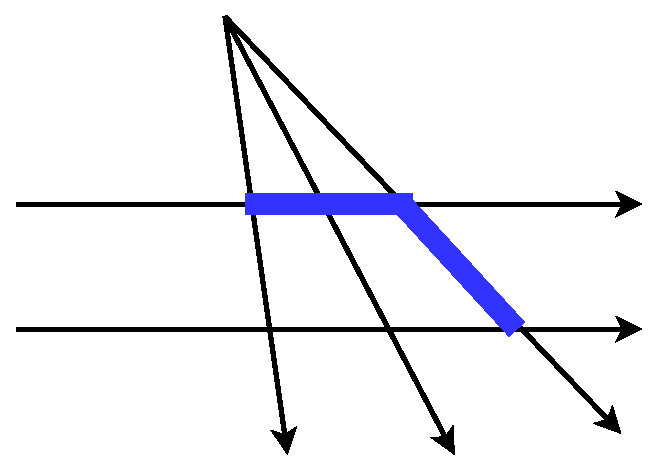
\includegraphics[width=\linewidth]{example1.pdf}
        \end{minipage}
        & 
         \begin{minipage}{0.3\textwidth}
            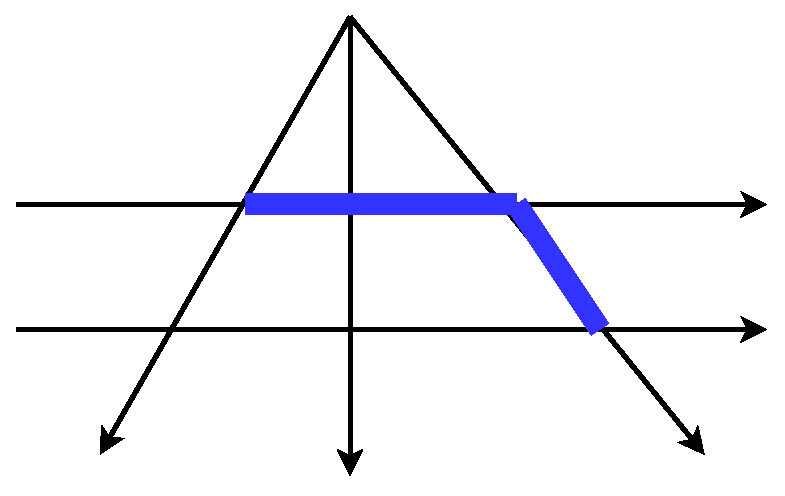
\includegraphics[width=\linewidth]{example2.pdf}
        \end{minipage}
        & 
         \begin{minipage}{0.3\textwidth}
            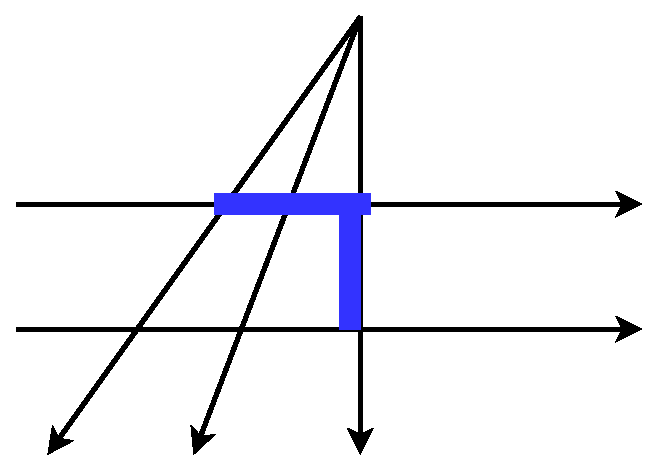
\includegraphics[width=\linewidth]{example3.pdf}
        \end{minipage} \\
        \begin{minipage}{0.3\textwidth}
            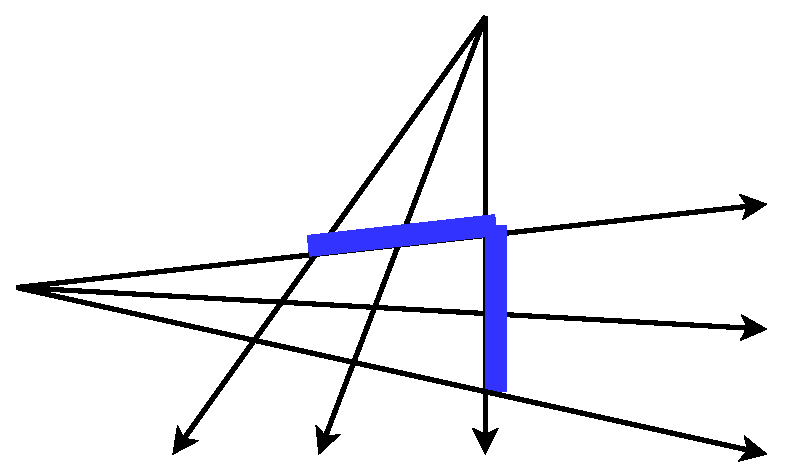
\includegraphics[width=\linewidth]{example4.pdf}
        \end{minipage} 
        & 
        \begin{minipage}{0.3\textwidth}
            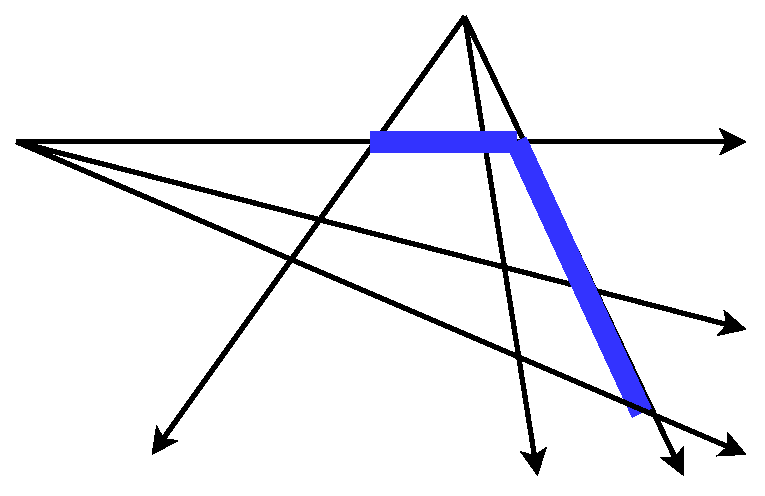
\includegraphics[width=\linewidth]{example5.pdf}
        \end{minipage} 
        &
        \begin{minipage}{0.3\textwidth}
            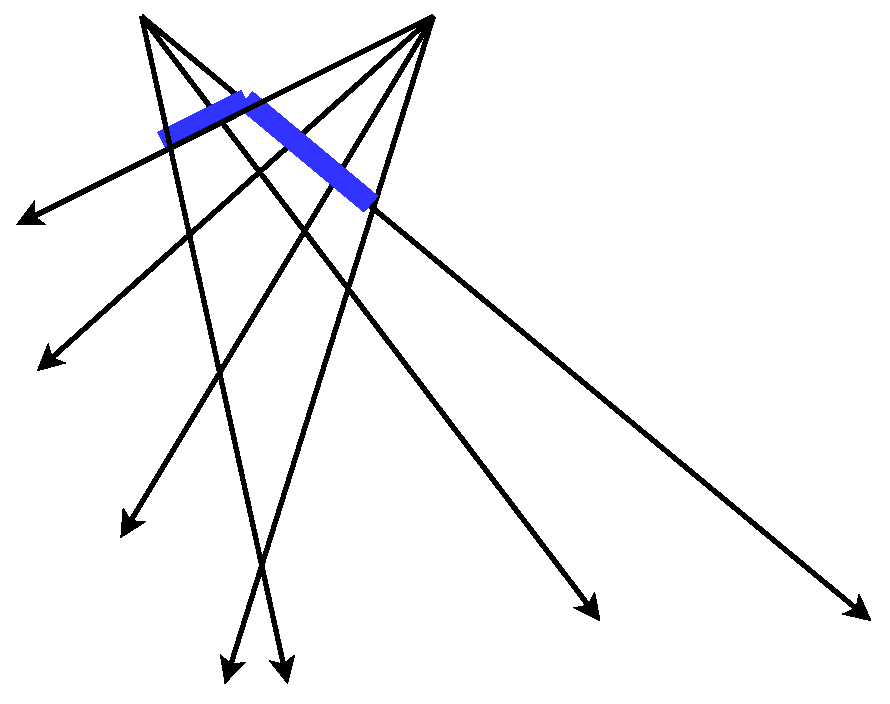
\includegraphics[width=\linewidth]{example6.pdf}
        \end{minipage} 
    \end{tabular}
    \begin{block}{Observation}
        Mid points are not used in the shortest path.
    \end{block}
\end{frame}

\begin{frame}{Faster solution}{Observation of some cases}
    \begin{block}{Assumption}
        The shortest path will never use the mid points. 
    \end{block}
    True ? Yes. kavitha etc \cite{kavitha2003shortest} proved it.
    \begin{tabular}{c c}
        \begin{minipage}{0.4\textwidth}
            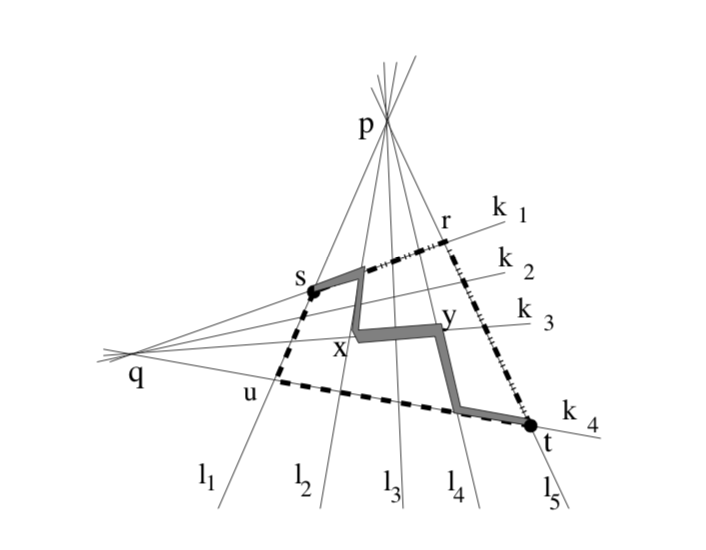
\includegraphics[width=\linewidth]{sut.png}
        \end{minipage}  
        &  
        \begin{minipage}{0.5\textwidth}
            \begin{theorem}
                The shortest s-t path is always one of s-u-t or s-r-t. 
            \end{theorem}
        \end{minipage} 
    \end{tabular}
    
\end{frame}


\begin{frame}{Faster solution}{Proof of kavitha's theorem}
    Let's start from a simple case. \\
    \begin{tabular}{c c}
        \begin{minipage}{0.4\textwidth}
            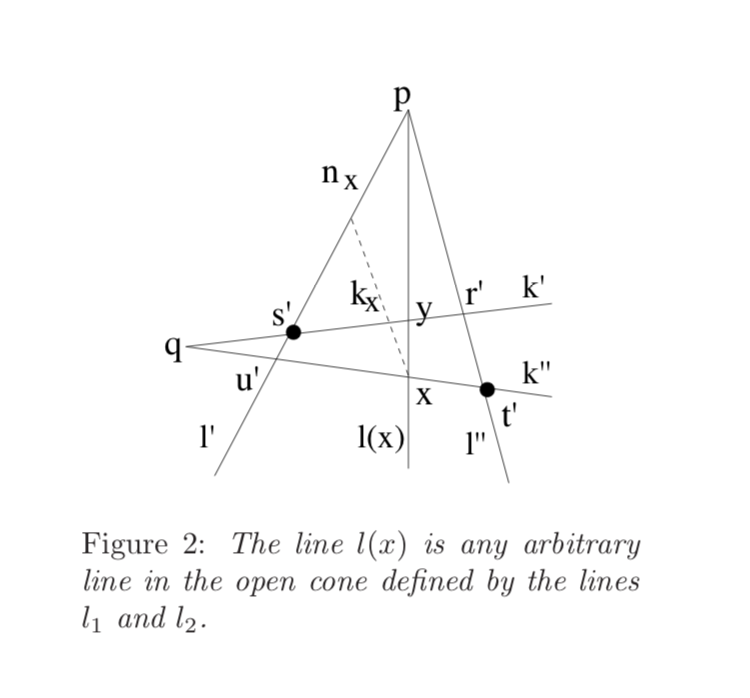
\includegraphics[width=\linewidth]{simple_proof.png}
        \end{minipage}  
        &  
        \begin{minipage}{0.5\textwidth}
            Path $s-y-x-t$, $s-u-x-t$ \\
            Assume $|suxt|$ is the shorter path \\
            \\
            Let $k$ be a point that satisfies $|sk| + |kx| = |su| + |ux|$ \\
            ($k$ lies between $s$ and $y$)
        \end{minipage} 
    \end{tabular}
\end{frame}

\begin{frame}{Faster solution}{Proof of kavitha's theorem}
    Let's start from a simple case. \\
    \begin{tabular}{c c}
        \begin{minipage}{0.4\textwidth}
            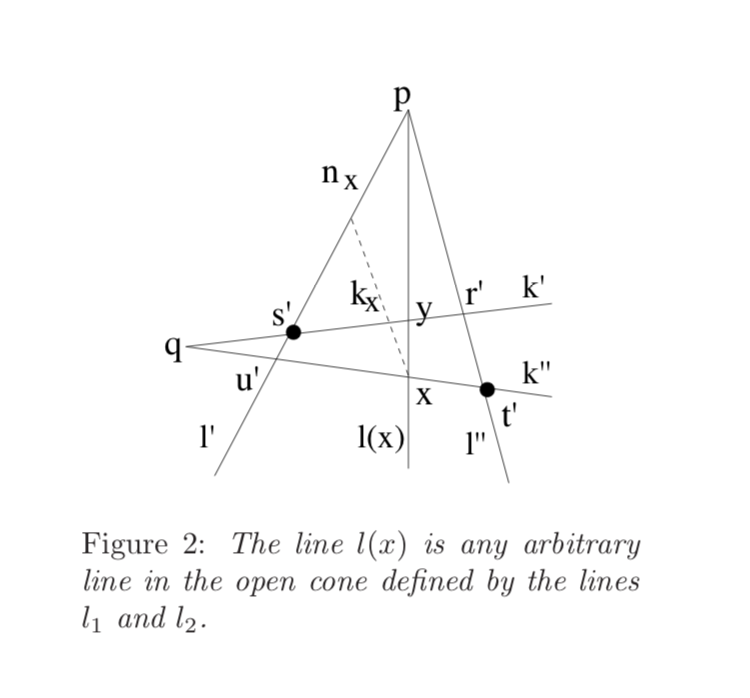
\includegraphics[width=\linewidth]{simple_proof.png}
        \end{minipage}  
        &  
        \begin{minipage}{0.5\textwidth}
            $|syxt| = |sy| + |yx| + |xt| = |sk| + |ky| + |yx| + |xt| $ \\
            $|suxt| = |su| + |ux| + |ut| $ \\ 
            \\
            Since $|sk| + |kx| = |su| + |ux|$ \\
            We have $|suxt|  = |sk| + |kx| + |ut| $ \\
            \\ 
            $|suxt| = |sk| + |ky| + |yx| + |xt| $ \\
            $|syxt| = |sk| + |kx| + |xt| $
        \end{minipage} 
    \end{tabular}
\end{frame}

\begin{frame}{Faster solution}{Proof of kavitha's theorem}
    Let's start from a simple case. \\
    \begin{tabular}{c c}
        \begin{minipage}{0.4\textwidth}
            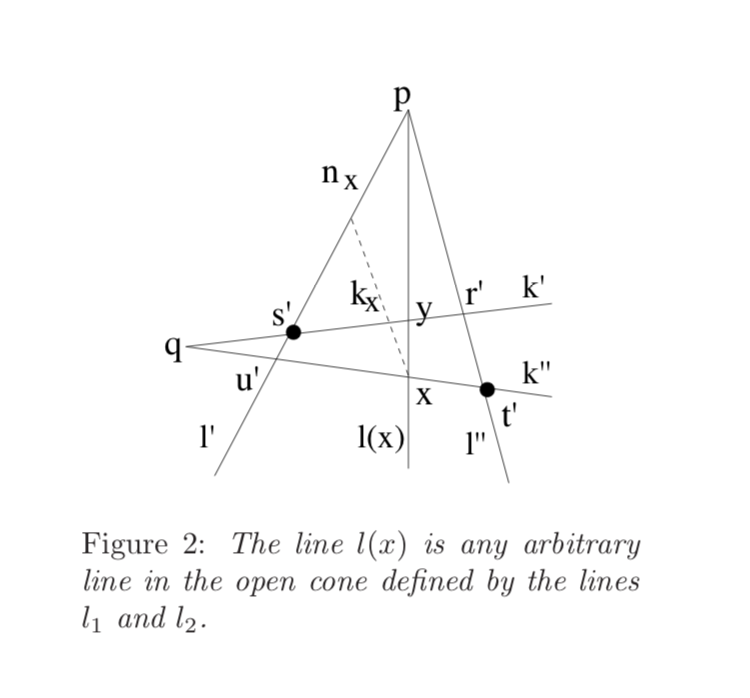
\includegraphics[width=\linewidth]{simple_proof.png}
        \end{minipage}  
        &  
        \begin{minipage}{0.5\textwidth}
            $|suxt| = |sk| + |ky| + |yx| + |xt| $ \\
            $|syxt| = |sk| + |kx| + |xt| $ \\
            $|suxt| - |syxt| = |ky| + |yx| - |kx| > 0 $ \\
            $$ |suxt| - |syxt| > 0 $$ 
            
            Similar proof can be done with $|suxt|$ and $|syxt|$.
        \end{minipage} 
    \end{tabular}
\end{frame}

\begin{frame}{Faster solution}{Proof of kavitha's theorem}
    Generalize to more edges \\
    Suppose the shortest s-t path (call it SP (s, t)) travels along line k1, then bends into li for some $2 \le i < n$ and then bends into $k$, $j$ for some $j > 1$. \\
    This contradicts kavitha's theorem applied to the lines l1 , li+1 , k1 , kj , and li.\\
    \begin{center}
    \begin{tabular}{c c}
        \begin{minipage}{0.4\textwidth}
            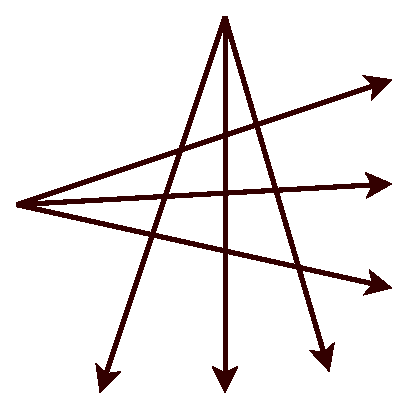
\includegraphics[width=\linewidth]{more_edges_1.pdf}
        \end{minipage}  
        &  
        \begin{minipage}{0.4\textwidth}
            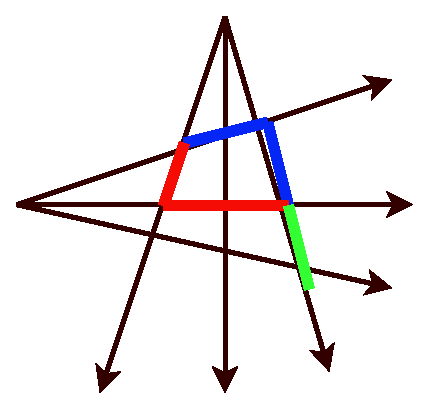
\includegraphics[width=\linewidth]{more_edges_2.pdf}
        \end{minipage} 
    \end{tabular}
    \end{center}
\end{frame}

\begin{frame}{Faster solution}{Kavitha's solution}
    Given two central points $k$ and $j$ and shoot $n$ and $m$ lines from the central respectively. To find the shortest path between left-up point to right-down point, the algorithm operates as following.
    \begin{enumerate}
        \item Find the lines with smallest and largest slop for $k$, name as ${lk}_1$ and ${lk}_2$
        \item Find the lines with smallest and largest slop for $j$, name as ${jn}_1$ and ${jm}_2$
        \item Compute the four intersection points. $A$: (${lk}_1$, ${jn}_1$),  $B$: (${lk}_1$, ${jm}_2$), $C$: (${lk}_2$, ${jn}_1$), $D$: (${lk}_2$, ${jm}_2$), 
        \item The shortest path is either $ABC$ or $ACD$
    \end{enumerate}
    Time complexity : $O(n)$
\end{frame}

% \begin{frame}{Faster solution}{Observation of a special case}
%     \begin{tabular}{c c}
%         \begin{minipage}{0.5\textwidth}
%             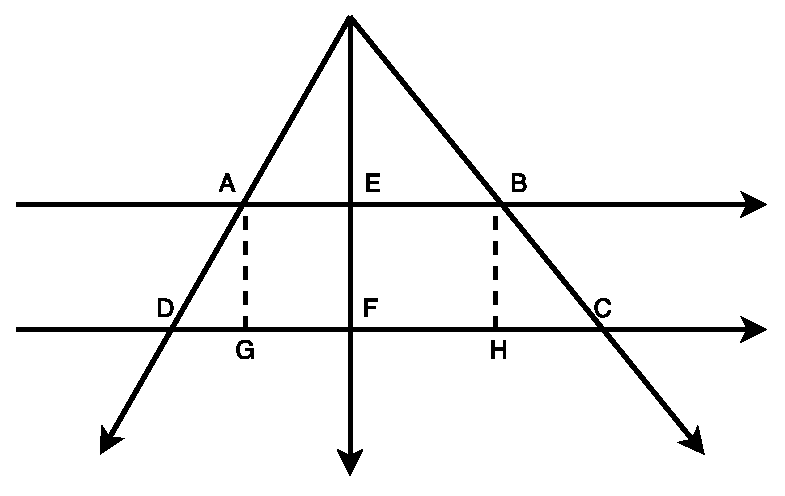
\includegraphics[width=\linewidth]{example.pdf}
%         \end{minipage}
%         & 
%          \begin{minipage}{0.4\textwidth}
%             Path1 : $A-E-F-C$ \\
%             Path2 : $A-E-B-C$ \\
%             Path3 : $A-D-F-C$ \\
%         \end{minipage}
%     \end{tabular}
% \end{frame}

% \begin{frame}{Faster solution}{Observation of a special case}
%     \begin{tabular}{c c}
%         \begin{minipage}{0.5\textwidth}
%             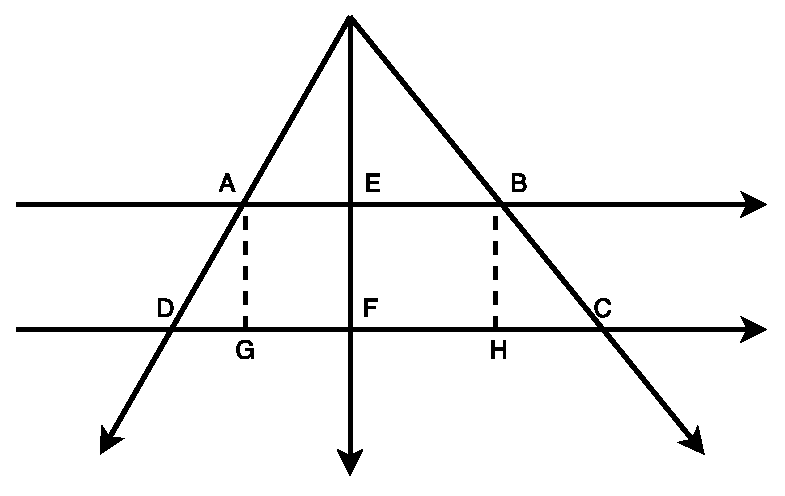
\includegraphics[width=\linewidth]{example.pdf}
%         \end{minipage}
%         & 
%          \begin{minipage}{0.4\textwidth}
%             Path1 : $A-E-F-C$ \\
%             Path2 : $A-E-B-C$ \\
%             $\text{Path1} - \text{Path2} \\
%                 = EF + FC - (EB + BC) \\
%                 = EF + (FH + FC) - (FH + BC) \\
%                 = EF + FC - BC > 0$ \\
%             $\text{Path1} > \text{Path2} $
%             If the line lies on right, Path on boundary 
%         \end{minipage}
%     \end{tabular}
% \end{frame}

% \begin{frame}{Faster solution}{Observation of a special case}
%     \begin{tabular}{c c}
%         \begin{minipage}{0.5\textwidth}
%             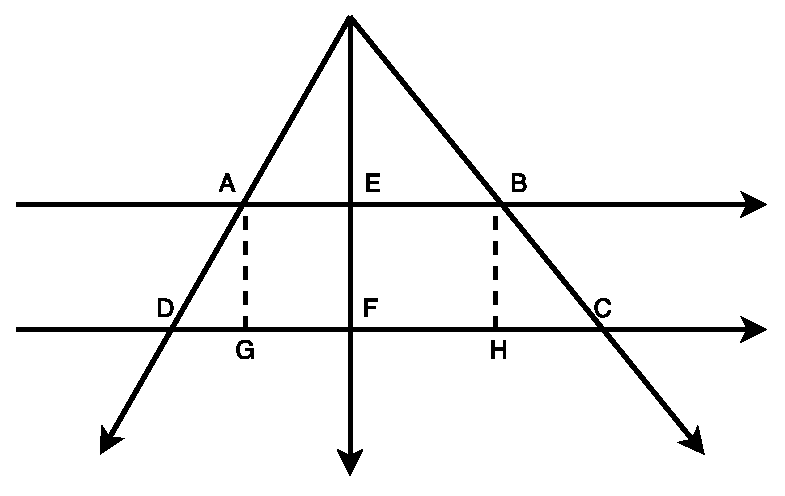
\includegraphics[width=\linewidth]{example.pdf}
%         \end{minipage}
%         & 
%          \begin{minipage}{0.4\textwidth}
%             Path1 : $A-E-F-C$ \\
%             Path3 : $A-E-B-C$ \\
%             $\text{Path1} - \text{Path3} \\
%                 = AE + EF - (AD + DF) \\
%                 = GF + EF - (AD + DG + GF) \\
%                 = EF - (AD + DG) < 0$ \\
%             $\text{Path1} < \text{Path3} $
                
%         \end{minipage}
%     \end{tabular}
% \end{frame}



% \begin{frame}{Blocks}
%     \begin{block}{Block Title}
%         You can also highlight sections of your presentation in a block, with it's own title
%     \end{block}
%     \begin{theorem}
%         There are separate environments for theorems, examples, definitions and proofs.
%     \end{theorem}
%     \begin{example}
%         Here is an example of an example block.
%     \end{example}
% \end{frame}

% Placing a * after \section means it will not show in the
% outline or table of contents.
% \section*{Summary}

\begin{frame}{Summary}
%   \begin{itemize}
%   \item
%     Conclude previous works on SPLA.
%     \item
%     The \alert{second main message} of your talk in one or two lines.
    
%   \end{itemize}
  
  \centering
    \begin{tabular}{|c|c|c|}
         \hline
         Method & \textbf{Constraints} & \textbf{Time complexity} \\
         \hline
         Naive & No & $O(n^2)$ \\
         \hline
         \cite{eppstein1997efficient} & Vertical and Horizontal & $O(n^{1.5})$, $O(nlgn)$ \\
         \hline
         \cite{eppstein1999shortest} & K slopes & $O(n + k^2)$ \\
         \hline
         \cite{bose1996approximating} & 2 approximation & $O(nlgn)$ \\
         \hline
         \cite{hart2001approximating} & $1 + \epsilon$ approximation & $O(nlogn + min(n, \frac{1}{\epsilon^2}) + \frac{1}{\epsilon} log \frac{1}{\epsilon})$\\
         \hline
         \hline
         Kavitha & \alert{No} & \alert{$O(n)$} \\
         \hline
    \end{tabular}
\end{frame}



% All of the following is optional and typically not needed. 
\appendix
\section<presentation>*{\appendixname}
\subsection<presentation>*{Reference}

\begin{frame}[allowframebreaks]
  \frametitle<presentation>{Reference}
   
  \bibliographystyle{abbrv}
    \bibliography{reference}
    \label{refer}
\end{frame}

\end{document}


